\documentclass[12pt, letterpaper]{article}
\usepackage[utf8]{inputenc}
\usepackage{graphicx}
\graphicspath{ {.} }
\usepackage{wrapfig}
 
\title{ASTP-720 Assignment 1}
\author{Brendan Drachler}
\date{\today}

\begin{document}
\maketitle
\section*{Problem 3}
For this problem, we want to find the full width at half maximum (FWHM), i.e., what is the width, $\frac{x}{r_c}$, when $N_e(x) = \frac{N_0}{2}$. To do so, we start from Eq. 14 in the assignment:

\begin{equation}
N_e(x) = \frac{N_0}{2} = N_0 [1 + (\frac{x}{r_c})^2 ]^{-\frac{1}{2}}
\end{equation}

In order to solve this with a root finding algorithm, we need to set our function equal to $0$. 

\begin{equation}
0 = [1 + (\frac{x}{r_c})^2 ]^{-\frac{1}{2}} - \frac{1}{2}
\end{equation}

We can now solve this with the bisection, newton, and secant method defined in root\_finder.py. One caveat is that for solving Newton's method, we will also need the value of the derivative. 

\begin{equation}
\frac{d}{dx} ([1 + (\frac{x}{r_c})^2 ]^{-\frac{1}{2}} - \frac{1}{2}) = \frac{x}{r_c} [1 + (\frac{x}{r_c})^2 ]^{-\frac{3}{2}} 
\end{equation}

Now the root finding algorithms can iterate to find the root. Each of them find, $\frac{x}{r_c} \approx -1.73205$. We can now ask how well each method does at converging as a function of the threshold. The threshold is a measure of how close we want to get to the root before we stop iterating. 

\begin{figure}[h]
\caption{The number of iterations we need to converge as a function of our chosen threshold.}
\centering
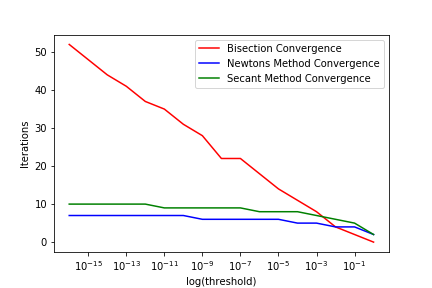
\includegraphics[width=0.7\textwidth]{threshold_vs_iterations}
\end{figure}

Fig. 1 shows that the bisection method tends to work best for large thresholds. This implies that if we do not want to strive for accuracy  $\leq 10^{-3}$, the bisection method will achieve appreciable accuracy in just a few iterations.  Meanwhile, Newton's method and the secant method both have a very similar rate of convergence at all thresholds. The secant method takes a few more iterations than Newton's method at all thresholds. This may be due to the particular function we are finding the root of. Therefore, I cannot conclude which is "better." 

\section{Problem 4}
In this problem, I've developed an algorithm to ray trace a particle's motion through a Gaussian spherical lens obeying:
\begin{equation}
x' = x [1 + \frac{\lambda^2 r_e N_0 D}{\pi a^2} e^{-(\frac{x}{a})^2}]
\end{equation}
Fig. 2 shows what an observer would see $1\ kpc$ from a Gaussian Lens.  It is easy to see that very little light would be focused towards the origin of the observer frame. Most of the light is focused away from the origin. Meanwhile, particle motion far away from the lens is unaffected like I would expect.
\begin{figure}[h]
\caption{Ray traced particle motion through a Gaussian Lens}
\centering
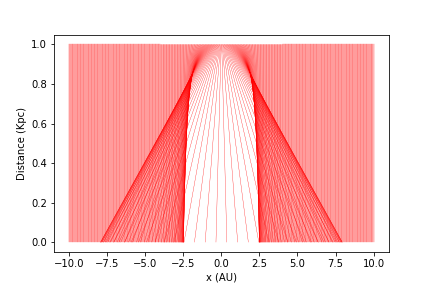
\includegraphics[width=0.7\textwidth]{gaussian_lense}
\end{figure}

\section{ Problem 5}
In this problem, I've developed an algorithm to ray trace a particle's motion through a pseudo-isothermal sphere by combining the following $3$ equations:
\begin{equation}
\frac{d N_e(x)}{dx} = -\frac{x N_0}{r_c^2 [1 + (\frac{x}{r_c})^2]^{\frac{3}{2}}}
\end{equation}
\begin{equation}
\theta_r(x) = \frac{\lambda^2 r_e }{2 \pi} \frac{d N_e(x)}{dx}
\end{equation}
\begin{equation}
x' = x - \theta_r(x) D
\end{equation}
Fig. 3 shows what an observer would see $1\ kpc$ from a pseudo-isothermal sphere.  It is easy to see that very little light would be focused towards the origin of the observer frame. Most of the light is focused away from the origin. Meanwhile, particle motion far away from the lens is unaffected like I would expect.

I cannot seem to find the density profile of a Gaussian lens, but I suspect the density falls off faster for the Gaussian lens than it does for the pseudo-isothermal sphere. This can be seen by comparing Fig. 2 and Fig. 3. The focusing regions are considerably farther apart for the pseudo-isothermal sphere than for the Gaussian lens. 
\begin{figure}[h]
\caption{Ray traced particle motion through a pseudo-isothermal sphere.}
\centering
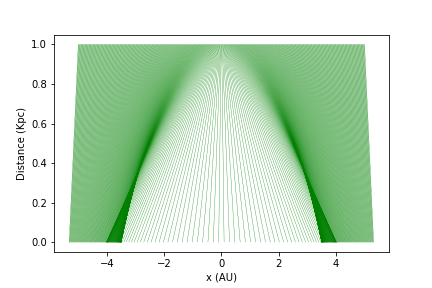
\includegraphics[width=0.7\textwidth]{pseudo_isothermal_sphere}
\end{figure}

\end{document}